% Chapter Template

\chapter{Implementation Methodology and Evaluation Strategy} % Main chapter title

\label{ChapterX} % Change X to a consecutive number; for referencing this chapter elsewhere, use \ref{ChapterX}

%----------------------------------------------------------------------------------------
%	SECTION 1
%----------------------------------------------------------------------------------------

This chapter provides an insight into the project implementation 
workflow, UI wireframe, data collection and processing methodology, 
and concludes with an evaluation strategy.

\section{Implementation Workflow}
The activity diagram displayed below provides a blueprint of the workflow 
that would be followed for the development phase commencing next semester. The wireframe illustrated in Appendix \ref{Wireframe} displays the expected general layout of the COVID-19 diagnosis portal.

\begin{figure}[H]
 \centering
 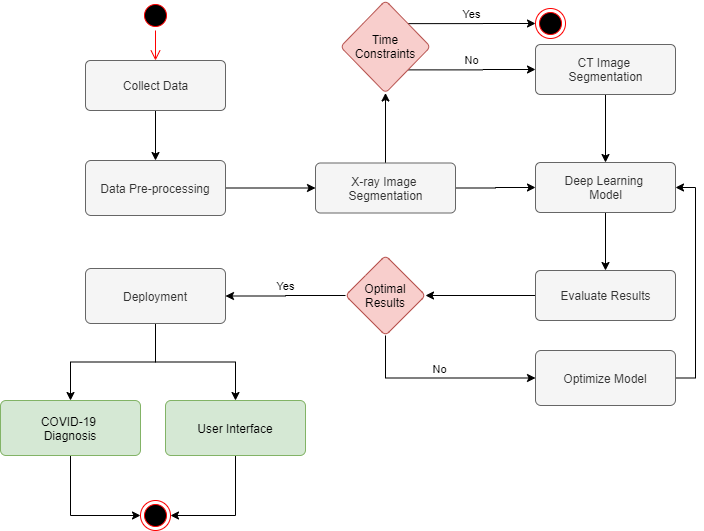
\includegraphics[width=15.5cm, height=7.4cm]{Images/Implementation Workflow.png}
 \decoRule
 \caption[Implementation Methodology]{Activity Diagram displaying the implementation workflow.}
 \label{fig:Implementation Methodology}
 \end{figure}
 
%  \vspace{-2em}
\section{Evaluation Strategy}
Table \ref{Evaluation Strategy} summarizes the methods and strategies used to evaluate each of the Functional Requirements described in Chapter \ref{Requirements Analysis}.

\begin{longtable}{| p{.10\textwidth} | p{.82\textwidth} |} 
\hline
\multicolumn{2}{|c|}{\textbf{Evaluation Strategy}}\\
\hline
\textbf{ID} & \textbf{Description}\\
\hline
FR-1 & \parbox[t]{12.3cm}{\textbf{X-ray Segmentation} \\ The lung segments produced from X-ray scans shall be evaluated based on its capability to identify possible ROIs.}\\\hline
FR-2 & \parbox[t]{12.3cm}{\textbf{CT Segmentation} \\ The lung segments produced from CT scans shall be evaluated based on its capability to identify possible ROIs.}\\\hline
FR-3 & \parbox[t]{12.3cm}{\textbf{COVID-19 Diagnosis using X-ray Scans} \\ The diagnosis results obtained after achieving FR-1 shall be evaluated against various statistical metrics such as Accuracy, Precision and Recall.}\\\hline
FR-4 & \parbox[t]{12.3cm}{\textbf{COVID-19 Diagnosis using CT Scans} \\ The diagnosis results obtained after achieving FR-2 shall be evaluated against various statistical metrics such as Accuracy, Precision and Recall.}\\\hline
FR-5 & \parbox[t]{12.3cm}{\textbf{Visualize Lung Region of Interest's} \\ The ROIs visualized correlates to the observed lung characteristics in COVID-19 patients.} \\\hline
FR-6 & \parbox[t]{12.3cm}{\textbf{Multi-class Diagnosis} \\ The diagnosis results obtained shall be evaluated against various statistical metrics such as Accuracy, Precision and Recall.}\\\hline
FR-7 & \parbox[t]{12.3cm}{\textbf{Web Interface} \\ The user interface developed shall evaluated based on the following metrics, that is, user-friendliness, consistency, familiarity, responsiveness, and intuitiveness\vspace{0.2em}}\\\hline
\caption{Evaluation Strategy}

  \label{tab:Evaluation Strategy}
  \end{longtable}
  
   
\section{Implementation Methodology}
A brief summary of the methodology that would be carried out in semester 2 as well as their evaluation is described in this section.
\subsection{Data Collection}
The two primary sources for collecting open source anonymized data would be the COVID-19 Kaggle datasets and the scans provided by Cohen et al. \cite{JMD2020} as seen from the literature review. The images obtained shall be separated into X-ray and CT scans separately and furthermore, on the basis of their labels.
\begin{itemize}
    \item \textbf{Testing} - Datasets which correspond to other lung diseases would also be used to analyse the generalizability of the model.
     \item \textbf{Evaluation} - Training would be conducted using  10-fold cross validation, followed by rigorous verification to prevent the model from either overfitting or underfitting.
\end{itemize}
\subsection{Data Pre-processing}
Before carrying out image segmentation for both X-ray and CT scans, all images in the training dataset shall undergo the same data pre-processing pipeline as per the model's input parameters.
\begin{itemize}
    \item \textbf{Testing} - The model would be tested on images  with different dimensions to ensure no input errors are caused.
     \item \textbf{Evaluation} - An input verification technique shall be applied to validate the provided training images before the deep learning workflow commences.
\end{itemize}
\subsection{Image Segmentation}
The provided training images, both X-ray and CT scans shall undergo segmentation such that the ROIs would be highlighted and lead to effective COVID-19 diagnosis
\begin{itemize}
    \item \textbf{Testing} - Multiple image segmentation techniques as suggested by the literature shall be used during the development phase to identify the one that yields the best results.
     \item \textbf{Evaluation} - All models used for experimentation purposes would be documented and the best would be utilized for final demonstration purposes.
\end{itemize}
\subsection{Model Optimization}
As observed in the literature review, multiple studies \cite{CXZ+2020, CYZ+2020, HLR+2020, YHQ+2020, GOM+2020, LLL+2020, CJL+2020, JSB+2020, SFY+2020} indicate variants of the U-Net architecture to be the best suited for CT scan segmentation whereas for X-rays, variants of ResNet and CNN seem to be ideal as per the research conducted \cite{ZXS+2020, AKP2020, GHT2020, LWA2020}.
\begin{itemize}
    \item \textbf{Testing} - Each of the proposed model variations shall be experimented with for testing purposes, and the results obtained shall be compared to existing literature. 
     \item \textbf{Evaluation} - The results obtained after tweaking the various hyper-parameters for each of the proposed models shall be tracked, thus being able to identify the most optimal set of values.
\end{itemize}
